\documentclass[a4paper,12pt]{article}

% Настройки языка и шрифтов
\usepackage[T2A]{fontenc}
\usepackage[utf8]{inputenc}
\usepackage[russian]{babel}
\usepackage{amsmath,amsfonts,amssymb}
\usepackage{graphicx}
\usepackage{color}
\usepackage{hyperref}
\usepackage{geometry}
\usepackage{csquotes}
\usepackage{indentfirst}
\usepackage{longtable}
\usepackage{booktabs}
\usepackage{float}

\geometry{left=3cm,right=1.5cm,top=2cm,bottom=2cm}

\begin{document}

% Титульный лист
\begin{titlepage}
    \centering
    {\fontsize{14pt}{16pt}\selectfont МОСКОВСКИЙ АВИАЦИОННЫЙ ИНСТИТУТ\\(НАЦИОНАЛЬНЫЙ ИССЛЕДОВАТЕЛЬСКИЙ УНИВЕРСИТЕТ)}\\[0.5cm]
    {\fontsize{12pt}{14pt}\selectfont Институт №8 «Компьютерные науки и прикладная математика»}\\[4cm]
    
    {\fontsize{16pt}{18pt}\selectfont \textbf{Лабораторные работы}}\\
    {\fontsize{14pt}{16pt}\selectfont \textbf{по курсу «Информационный поиск»}}\\[5cm]
    
    \vfill
    \begin{flushright} 
        \begin{minipage}{0.51\textwidth}
            Выполнил: Галкин Алексей Дмитриевич\\
            Группа: М8О-408Б-22\\
            Преподаватель: Кухтичев Антон Алексеевич
        \end{minipage}
    \end{flushright}
    
    \vfill
    {\large Москва, 2026}
\end{titlepage}

\tableofcontents
\newpage

\section{Введение}
В рамках курса «Информационный поиск» была разработана поисковая система, включающая подсистемы сбора данных (краулер), обработки текста (токенизация, стемминг), индексации и поиска. Сбор данных и веб-интерфейс был реализован на языке Golang, а ядро системы (индексация и поиск) реализовано на языке C++ с использованием собственных структур данных (вектор, хеш-таблица) в соответствии с требованиями курса.

\section{Лабораторная работа №1: Добыча корпуса документов}

\subsection{Цель работы}
Собрать и проанализировать корпус текстовых документов объемом не менее 30 000 статей для последующего использования в поисковой системе.

\subsection{Описание источников}
В качестве предметной области была выбрана тематика живых существ, а именно животные, растения и грибы. Источниками данных послужили:
\begin{itemize}
    \item русскоязычный раздел Википедии. Выли выбраны 3 категории: Животные по алфавиту, Растения по алфавиту, Грибы по алфавиту. Собрано 65,000 статей.
    \item журнал о животных (https://animaljournal.ru/)  Собрано 282 статей.
\end{itemize}

\subsection{Статистика корпуса}
\begin{table}[H]
\centering
\begin{tabular}{|l|c|}
\hline
\textbf{Параметр} & \textbf{Значение} \\
\hline
Количество документов (всего) & 65,282 \\
\hline
\quad из Википедии & 65,000 \\
\hline
\quad из animaljournal & 282 \\
\hline
Формат хранения & JSONL \\
\hline
Язык & русский (с включениями из других языков) \\
\hline
\end{tabular}
\caption{Статистика собранного корпуса}
\end{table}

\section{Лабораторная работа №2: Поисковый робот}

\subsection{Цель работы}
Разработать поисковый робот для автоматического сбора документов, проверки свежести и наличием задержки.

\subsection{Архитектура и стек технологий}
Робот реализован на языке \textbf{Golang} с использованием MongoDB. Основные библиотеки: net/http, golang.org/x/net/html, crypto/sha256.
Для обеспечения надёжности работы в HTTPClient реализован механизм повторных попыток с экспоненциальной задержкой (retry logic) и ограничение частоты запросов (rate limiting) с использованием мьютексов для потокобезопасности.

Архитектура построена по принципу разделения ответственности и включает три основных уровня: уровень представления (конфигурация и точка входа), уровень управления (центральный менеджер Crawler) и уровень источников данных (клиенты для различных сайтов).

\subsection{Алгоритм работы}
\begin{itemize}
    \item \textbf{Инициализация}: чтение конфигурации из YAML файла, подключение к MongoDB, создание уникальных индексов для предотвращения дубликатов.
    \item \textbf{Управление источниками}: Проверка наличия активных источников в конфигурации и запуск процесса обхода.
    \item \textbf{Обход Википедии}:
    \begin{itemize}
        \item Для каждой категории:
        \begin{itemize}
            \item Формирование API-запроса к MediaWiki API.
            \item Получение списка страниц в категории (по 500 записей за запрос).
            \item Извлечение page\_id и названий страниц.
        \end{itemize}
        \item Обработка пагинации через параметр cmcontinue.
        \item Для каждой страницы проверка наличия в базе данных по page\_id, загрузка HTML.
        \item Сохранение в MongoDB.
    \end{itemize}
    \item \textbf{Обход AnimalJournal}:
    \begin{itemize}
            \item Загрузка первой страницы категории.
            \item Извлечение ссылок на статьи по CSS-классу post\_title и поиск ссылки на следующую страницу в блоке пагинации.
            \item Добавка каждой страницы пагинации в очередь на обработку. Предотвращение повторного посещения через seenPages.
            \item Генерация числового ID через хеширование URL (FNV-32a) для каждой ссылки на статью.
            \item Загрузка каждой HTML страницы статьи.
            \item Сохранение в MongoDB
    \end{itemize}
    \item \textbf{Контроль дубликатов}:
    \begin{itemize}
            \item Перед загрузкой: Для Википедии проверка page\_id, для AnimalJournal URL-хеша.
            \item Перед сохранением: Вычисление SHA256 от HTML-содержимого и проверка существования документа с таким же хешем.
    \end{itemize}
\end{itemize}

\subsection{Формат хранения данных}
Документы хранятся в MongoDB в коллекции documents со следующей структурой:
\begin{itemize}
    \item page\_id (int) — уникальный идентификатор страницы.
    \item title (string) — заголовок документа.
    \item url (string) — канонический URL (очищенный от UTM-меток).
    \item html (string) — полное HTML-содержимое страницы.
    \item sha256 (string) — контрольная сумма содержимого.
    \item category (string) — категория или источник.
    \item downloaded\_at (datetime) — время загрузки.
\end{itemize}
Для экспорта данных используется формат JSON Lines (JSONL), где каждый документ представлен отдельной строкой в UTF-8-кодировке. Это обеспечивает возможность потоковой обработки файлов любого размера без загрузки в память целиком.
При перезапуске робот проверяет наличие уже загруженных документов в базе данных и пропускает их, что обеспечивает идемпотентность операций и позволяет докачивать только новые страницы.

\section{Лабораторная работа №3: Токенизация}

\subsection{Цель работы}
Реализовать разбиение текста на токены (слова), которые будут использоваться при индексации Нужно будет учитывать особенности русского языка и многобайтовой кодировки UTF-8.

\subsection{Основные компоненты}
Токенизатор реализован в виде класса Tokenizer на C++. Основная функция - tokenize, которая принимает строку и возвращает вектор std::string токенов.

Алгоритм работы:
\begin{itemize}
    \item Обработка UTF-8 - Для каждого байта определяется, является ли он началом символа, и вычисляется полная длина символа в байтах. Это позволяет избежать "разрыва" многобайтовых символов при обработке.
    \item Распознавание буквенных символов.
    \item Приведение к нижнему регистру.
    \item Алгоритм выделения токенов
    \begin{itemize}
        \item Текст сканируется посимвольно (с учётом реальной длины символов в байтах).
        \item При обнаружении буквы она добавляется в буфер текущего слова.
        \item При обнаружении не-буквы (пробел, знак препинания и т.д.) текущее слово сохраняется в массив токенов, а буфер очищается.
        \item Короткие слова (менее двух символов) отбрасываются как незначимые.
    \end{itemize}
\end{itemize}


\subsection{Особенности реализации}
\begin{itemize}
    \item Эффективность
    \begin{itemize}
        \item Алгоритм однопроходный - текст сканируется один раз;
        \item Не создаются промежуточные копии текста;
        \item Используется минимальное количество выделений памяти;
    \end{itemize}
    \item Устойчивость к ошибкам
    \begin{itemize}
        \item При обнаружении некорректной UTF-8 последовательности алгоритм продолжает работу;
        \item Нераспознанные символы обрабатываются как разделители;
    \end{itemize}
    \item Расширяемость
    \begin{itemize}
        \item Легко добавить поддержку других алфавитов (например, латиницы с диакритикой)
    \end{itemize}
\end{itemize}

\section{Лабораторная работа №4: Стемминг}

\subsection{Цель работы}
Реализовать морфологическую нормализацию (стемминг) для улучшения полноты поиска. 

\subsection{Метод решения}
Реализован \textbf{алгоритм Портера} для русского языка на C++. Алгоритм последовательно применяет ряд правил для отсечения суффиксов и окончаний.

Перед применением правил в слове выделяются специальные области. Это необходимо, чтобы отсекать только суффиксы, не затрагивая корень.

Области:
\begin{enumerate}
    \item RV - область после первой гласной буквы в слове
    \item R1 - область после первой гласной, которая следует за согласной
    \item R2 - область внутри R1, начинающаяся после следующей гласной
\end{enumerate}

Таблица суффиксов:
\begin{enumerate}
    \item Суффиксы причастий и деепричастий: "вшись", "вши", "в"
    \item Суффиксы прилагательных: "ими", "ыми", "его", "ого" и др.
    \item Суффиксы причастий: "ем", "нн", "вш", "ющ"
    \item Возвратные суффиксы: "ся", "сь"
    \item Простые глагольные суффиксы: "ете", "нно", "йте", "ла", "ло" и др.
    \item Сложные глагольные суффиксы: "ейте", "уйте", "ыли", "ыть", "ит" и др.
    \item Суффиксы существительных: "иями", "ями", "ами", "ев", "ов", "ие", "ье" и др.
    \item Суффиксы превосходной степени: "ейше", "ейш" 
\end{enumerate}

Последовательность применений правил:
\begin{enumerate}
    \item Обработка причастий и деепричастий (сначала выполняются более специфические правила)
    \item Удаление возвратных суффиксов
    \item Обработка прилагательных (пробуются суффиксы прилагательных, потом причастий)
    \item Обработка глаголов
    \item Обработка существительных
    \item Удаление конечного "и"
    \item Обработка суффиксов "ость"/"ост" (только в области R2)
    \item Обработка суффиксов превосходной степени
    \item Нормализация двойного "н"
    \item Удаление мягкого знака в области RV
\end{enumerate}

\section{Лабораторная работа №5: Закон Ципфа}

\subsection{Цель работы}
Проверить выполнение закона Ципфа на собранном корпусе документов.

\subsection{Теоретические основы}

\textbf{Закон Ципфа} утверждает, что частота слова в корпусе текстов обратно пропорциональна его рангу:

\[ f(r) = \frac{C}{r} \]

где $f(r)$ --- частота термина с рангом $r$, $C$ --- константа, зависящая от корпуса.

В логарифмической шкале закон Ципфа представляет собой прямую линию с наклоном $-1$:

\[ \log f(r) = \log C - \log r \]

Более точное приближение даёт обобщённый закон Ципфа--Мандельброта:
\[ f(r) = \frac{C}{(r + b)^a} \]
где $a$ и $b$ --- параметры, подбираемые по реальным данным.

\subsection{Реализация анализатора}

Класс \texttt{ZipfAnalyzer} реализован на C++ и выполняет следующие функции:
\begin{enumerate}
    \item Подсчёт частот всех терминов после стемминга с использованием собственной хеш-таблицы \texttt{StringMap}
    \item Сортировка терминов по убыванию частоты (сортировка вставками)
    \item Присвоение рангов
    \item Записывает полученные результаты в CSV-файл со столбцами:
    \begin{enumerate}
        \item rank
        \item term
        \item frequency
        \item log\_rank
        \item log\_frequency
    \end{enumerate}
\end{enumerate}
Для  построения графика был реализован скрипт на Python
\subsection{Результаты}

\begin{figure}[H]
\centering
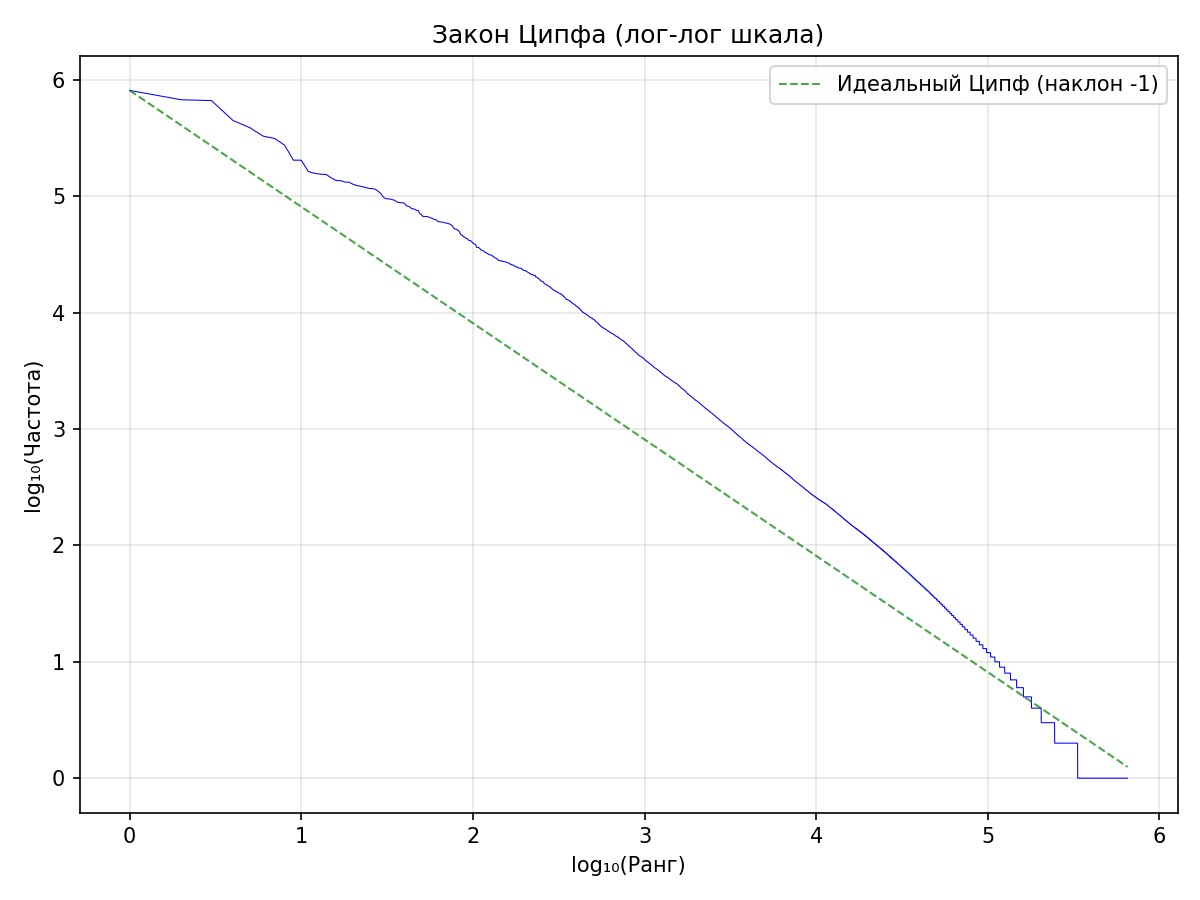
\includegraphics[width=0.9\textwidth]{images/zipf_plot.png}
\caption{Распределение частот терминов (закон Ципфа)}
\end{figure}

\textbf{Топ-10 самых частотных слов:}
\begin{table}[H]
\centering
\begin{tabular}{|c|l|r|}
\hline
\textbf{Ранг} & \textbf{Терм} & \textbf{Частота} \\
\hline
1 & в & 815668 \\
2 & и & 677538 \\
3 & на & 666632 \\
4 & с & 449801 \\
5 & вид & 314956 \\
6 & род & 205073 \\
7 & год & 157755 \\
8 & семейств & 154289 \\
9 & из & 143941 \\
10 & без & 136810 \\
\hline
\end{tabular}
\caption{Топ-10 частотных терминов}
\end{table}

Согласно закону Ципфа: $f \approx \frac{C}{r^s}$, где $s \approx 1$.

Полученный график демонстрирует линейную зависимость с наклоном, близким к $-1$, что в целом подтверждает выполнение закона Ципфа для собранного корпуса научных текстов.

\subsection{Причины расхождений}
На графике наблюдаются характерные отклонения от идеального закона Ципфа:

\textbf{1. Область высоких рангов (частотные слова):}
\begin{itemize}
    \item Cлишком много слов с очень высокой частотой. Это "обязательные" термины, которые есть везде.
\end{itemize}

\textbf{2. Область низких рангов (редкие слова):}
\begin{itemize}
    \item Наблюдается \textbf{ступенчатость} --- много слов с частотой 1, 2, 3.
    \item Частота \textbf{выше} предсказанной (хвост толще).
    \item Причина: огромное количество уникальных терминов
\end{itemize}

\textbf{3. Средняя область:}
\begin{itemize}
    \item Хорошее соответствие закону Ципфа.
    \item Это типично для естественных текстов.
\end{itemize}

\subsection{Выводы}
Закон Ципфа выполняется для собранного корпуса с типичными отклонениями, характерными для научных текстов. Отклонения объясняются особенностями предметной области.

\section{Лабораторная работа №6: Построение булева индекса для коллекции документов}

\subsection{Цель работы}
Разработать и реализовать инвертированный индекс для поддержки булева поиска в коллекции веб-документов. Индекс должен храниться в бинарном формате с оптимизацией для эффективного выполнения поисковых запросов.

\subsection{Структура документа после обработки}
Исходный документ (HTML-страница) проходит через конвейер обработки, в результате чего формируется внутреннее представление:

\begin{enumerate}
    \item \textbf{Извлечение текста}: из HTML удаляются все теги, скрипты и стили. Остаётся "чистый" текст.
    \item \textbf{Токенизация}: текст разбивается на отдельные слова (токены) с учётом UTF-8 кодировки.
    \item \textbf{Стемминг}: каждый токен приводится к его основе с помощью стеммера Портера для русского языка.
\end{enumerate}

В результате документ представляется как последовательность термов (стеммированных токенов). Для каждого терма сохраняется информация о его позиции(ях) в документе, что позволяет в дальнейшем реализовать поиск по фразам и ранжирование по близости термов.

\subsection{Архитектура индексатора}

Индексатор реализован на языке C++ без использования STL-контейнеров. Все структуры данных разработаны самостоятельно для обеспечения полного контроля над памятью и форматом хранения.

\subsubsection{Собственные структуры данных}

\begin{itemize}
    \item \textbf{HashMap}: хеш-таблица с открытой адресацией для хранения словаря термов. Ключом является строка терма, значением — указатель на постинг-лист. При коллизиях используется линейное пробирование. Размер таблицы динамически увеличивается при достижении коэффициента загрузки 0.75.

    \item \textbf{DynArray}: динамический массив для хранения последовательностей чисел (doc\_id, позиции термов). Реализует автоматическое расширение с коэффициентом 2 при заполнении. Поддерживает вставку в конец за амортизированное O(1).
\end{itemize}

\subsubsection{Процесс индексации}

Индексация выполняется в один проход по коллекции документов:

\begin{enumerate}
    \item Документы читаются последовательно из JSONL-файла.
    \item Для каждого документа:
    \begin{itemize}
        \item Извлекается текст из HTML (функция stripHTML).
        \item Выполняется токенизация с приведением к нижнему регистру.
        \item Каждый токен пропускается через стеммер.
        \item Для каждого уникального терма в документе формируется постинг, содержащий doc\_id, частоту терма и список позиций.
        \item Постинг добавляется в хеш-таблицу (если терм новый — создаётся новый постинг-лист).
    \end{itemize}
\end{enumerate}

Важная особенность: поскольку документы обрабатываются в порядке возрастания doc\_id (от 0 до N-1), постинг-листы автоматически получаются отсортированными по doc\_id. Это позволяет избежать дополнительной сортировки при сохранении индекса.

\subsubsection{Бинарный формат индекса}

Индекс сохраняется в единый бинарный файл следующей структуры:

\begin{verbatim}
[0-7]    Magic: "IRIDX003" (8 байт) — сигнатура и версия формата

[8-11]   NumDocs: uint32 — количество документов

[12...]  Документы (NumDocs записей):
         - docId: uint32
         - title_len: uint32
         - title: char[title_len]
         - url_len: uint32
         - url: char[url_len]

[...]    NumTerms: uint32 — количество уникальных термов

[...]    Термы (NumTerms записей):
         - term_len: uint32
         - term: char[term_len]
         - numPostings: uint32
         - Постинги (numPostings записей):
           * docId: uint32
           * count: uint32 (частота терма в документе)
           * snippet_len: uint32
           * snippet: char[snippet_len]
\end{verbatim}

\textbf{Преимущества формата:}
\begin{itemize}
    \item Простота реализации и отладки
    \item Компактное представление
    \item Возможность загрузить весь индекс одной операцией чтения
\end{itemize}
\subsection{Результаты индексации}

Индексация выполнялась на коллекции из 65,136 документов (смесь русскоязычных статей из Википедии и AnimalJournal.ru).

\begin{table}[H]
\centering
\begin{tabular}{|l|r|}
\hline
\textbf{Параметр} & \textbf{Значение} \\
\hline
Количество уникальных термов & 652,748 \\
\hline
Размер файла словаря (index.bin) & 2.8 Гб \\
\hline
\end{tabular}
\caption{Статистические характеристики булева индекса}
\end{table}

\subsection{Анализ масштабируемости}

\textbf{Текущие ограничения:}
\begin{itemize}
    \item Индекс строится полностью в оперативной памяти, что ограничивает максимальный размер коллекции доступным RAM.
    \item Однопоточная обработка не использует преимущества многоядерных процессоров.
    \item При индексации используется наивный подход к выделению памяти.
\end{itemize}

\textbf{Прогноз масштабирования:}
\begin{itemize}
    \item \textbf{10× данных (650k документов)}: потребуется ~2.5-3 ГБ RAM, что всё ещё выполнимо на современных машинах. Время индексации ~7-8 минут.
    \item \textbf{100× данных (6.5M документов)}: потребуется ~25-30 ГБ RAM, что превышает типичные возможности desktop-систем. Потребуется внешняя сортировка (external merge sort) или распределённая индексация.
    \item \textbf{1000× данных (65M документов)}: необходим распределённый подход (MapReduce, Apache Spark) с индексацией на кластере.
\end{itemize}

\textbf{Возможные оптимизации:}
\begin{enumerate}
    \item \textbf{Многопоточная токенизация}: разделение документов между потоками с последующим слиянием частичных индексов.
    \item \textbf{Внешняя сортировка}: при нехватке памяти постинг-листы сортируются на диске.
    \item \textbf{Блочное сжатие}: применение более эффективных алгоритмов сжатия (LZ4, Zstd) для постинг-листов.
    \item \textbf{Инкрементальная индексация}: возможность добавления новых документов без перестройки всего индекса.
\end{enumerate}

\section{Лабораторная работа №7: Реализация булева поиска}

\subsection{Цель работы}
Разработать поисковый движок, выполняющий булевы запросы (AND, OR, NOT) по построенному индексу, и предоставить интерфейсы для взаимодействия (командная строка и веб-интерфейс).

\subsection{Синтаксис запросов}

Парсер запросов поддерживает следующий синтаксис (инспирированный поисковыми системами):

\begin{itemize}
    \item \textbf{AND} — логическое И (пересечение множеств).
    \item \textbf{OR} — логическое ИЛИ (объединение множеств).
    \item \textbf{NOT} — логическое НЕ (дополнение множества).
    \item \textbf{Скобки} — изменение приоритета операций.
\end{itemize}

\textbf{Примеры запросов:}
\begin{itemize}
    \item \texttt{кошка AND собака} — документы, содержащие оба слова
    \item \texttt{кошка OR собака} — документы, содержащие хотя бы одно из слов
    \item \texttt{кошка AND NOTсобака} — документы с "кошка", но без "собака"
    \item \texttt{(кошка OR собака) AND NOT мышь} — документы с кошкой или собакой, но без мыши
\end{itemize}

\subsection{Архитектура поискового движка}

\subsubsection{Компоненты}

\begin{enumerate}
    \item \textbf{Загрузчик индекса}: читает бинарные файлы индекса и загружает их в память:
    \begin{itemize}
        \item Словарь загружается в хеш-таблицу для быстрого доступа по терму
        \item Постинг-листы могут загружаться полностью или отображаться через memory-mapped I/O
        \item Информация о документах загружается в массив для быстрого доступа по doc\_id
    \end{itemize}

    \item \textbf{Парсер запросов}: реализован методом рекурсивного спуска:
    \begin{itemize}
        \item \texttt{parseExpression()} — обрабатывает операторы OR (самый низкий приоритет)
        \item \texttt{parseTerm()} — обрабатывает операторы AND
        \item \texttt{parseFactor()} — обрабатывает операторы NOT и атомы (термы или скобки)
    \end{itemize}

    \item \textbf{Исполнитель запросов}: выполняет операции над множествами документов:
    \begin{itemize}
        \item Для каждого терма из индекса извлекается список doc\_id
        \item Выполняются операции пересечения, объединения и дополнения
        \item Результат сортируется для вывода
    \end{itemize}
\end{enumerate}

\subsection{Реализация парсера рекурсивного спуска}

Парсер обрабатывает запрос в соответствии с формальной грамматикой:

\begin{verbatim}
<expression> ::= <term> ( 'OR' <term> )*
<term>       ::= <factor> ( 'AND' <factor> )*
<factor>     ::= 'NOT' <factor> | '(' <expression> ')' | <word>
<word>       ::= последовательность букв (латиница или кириллица)
\end{verbatim}

\textbf{Преимущества рекурсивного спуска:}
\begin{itemize}
    \item Прямое отображение грамматики на код
    \item Легко расширять (добавление новых операторов)
    \item Понятная обработка приоритетов
    \item Естественная поддержка скобок
\end{itemize}

\subsection{Примеры выполнения запросов}

Для тестирования использовалась коллекция из 65,282 документов.

\begin{table}[H]
\centering
\begin{tabular}{|l|c|l|}
\hline
\textbf{Запрос} & \textbf{Результатов} \\
\hline
\texttt{кенгуру} & 228 \\
\hline
\texttt{кенгуру AND австралия} & 137 \\
\hline
\texttt{кенгуру OR коала} & 244 \\
\hline
\texttt{кенгуру NOT коала} & 220 \\
\hline
\texttt{(кенгуру OR вомбат) AND австралия} & 149 \\
\hline
\texttt{кошка AND собака AND мышь} & 46 \\
\hline
\texttt{NOT кенгуру} & 65054 \\
\hline
\end{tabular}
\caption{Примеры выполнения запросов}
\end{table}

\subsection{Интерфейсы поиска}

\subsubsection{Командная строка (CLI)}

\begin{verbatim}
# Пакетный режим
$ ./search -index /path/to/index -query "кенгуру && австралия"
Query: кенгуру AND австралия
Results: 137 documents
-1143397447     Динго – собака Австралии, которая одичала. Описание и фото собаки динго https://animaljournal.ru/article/dingo_sobaka_avstralii
-93928591       Большой рыжий кенгуру – гигант Австралии. Описание и фото рыжего кенгуру        https://animaljournal.ru/article/kenguru
8743    Млекопитающие   https://ru.wikipedia.org/wiki/%D0%9C%D0%BB%D0%B5%D0%BA%D0%BE%D0%BF%D0%B8%D1%82%D0%B0%D1%8E%D1%89%D0%B8%D0%B5
16232   Утконос https://ru.wikipedia.org/wiki/%D0%A3%D1%82%D0%BA%D0%BE%D0%BD%D0%BE%D1%81
61824   Сумчатые        https://ru.wikipedia.org/wiki/%D0%A1%D1%83%D0%BC%D1%87%D0%B0%D1%82%D1%8B%D0%B5
80816   Гребнистый крокодил     https://ru.wikipedia.org/wiki/%D0%93%D1%80%D0%B5%D0%B1%D0%BD%D0%B8%D1%81%D1%82%D1%8B%D0%B9_%D0%BA%D1%80%D0%BE%D0%BA%D0%BE%D0%B4%D0%B8%D0%BB
84474   Сумчатый волк   https://ru.wikipedia.org/wiki/%D0%A1%D1%83%D0%BC%D1%87%D0%B0%D1%82%D1%8B%D0%B9_%D0%B2%D0%BE%D0%BB%D0%BA
84733   Динго   https://ru.wikipedia.org/wiki/%D0%94%D0%B8%D0%BD%D0%B3%D0%BE
86227   Коала   https://ru.wikipedia.org/wiki/%D0%9A%D0%BE%D0%B0%D0%BB%D0%B0
100661  Двурезцовые сумчатые    https://ru.wikipedia.org/wiki/%D0%94%D0%B2%D1%83%D1%80%D0%B5%D0%B7%D1%86%D0%BE%D0%B2%D1%8B%D0%B5_%D1%81%D1%83%D0%BC%D1%87%D0%B0%D1%82%D1%8B%D0%B5
147036  Австралийская ехидна    https://ru.wikipedia.org/wiki/%D0%90%D0%B2%D1%81%D1%82%D1%80%D0%B0%D0%BB%D0%B8%D0%B9%D1%81%D0%BA%D0%B0%D1%8F_%D0%B5%D1%85%D0%B8%D0%B4%D0%BD%D0%B0
148095  Бандикуты       https://ru.wikipedia.org/wiki/%D0%91%D0%B0%D0%BD%D0%B4%D0%B8%D0%BA%D1%83%D1%82%D1%8B
148716  Кенгуровые      https://ru.wikipedia.org/wiki/%D0%9A%D0%B5%D0%BD%D0%B3%D1%83%D1%80%D0%BE%D0%B2%D1%8B%D0%B5
149229  Мускусная кенгуровая крыса      https://ru.wikipedia.org/wiki/%D0%9C%D1%83%D1%81%D0%BA%D1%83%D1%81%D0%BD%D0%B0%D1%8F_%D0%BA%D0%B5%D0%BD%D0%B3%D1%83%D1%80%D0%BE%D0%B2%D0%B0%D1%8F_%D0%BA%D1%80%D1%8B%D1%81%D0%B0
149443  Кенгуровые крысы (сумчатые)     https://ru.wikipedia.org/wiki/%D0%9A%D0%B5%D0%BD%D0%B3%D1%83%D1%80%D0%BE%D0%B2%D1%8B%D0%B5_%D0%BA%D1%80%D1%8B%D1%81%D1%8B_%28%D1%81%D1%83%D0%BC%D1%87%D0%B0%D1%82%D1%8B%D0%B5%29
149504  Потору  https://ru.wikipedia.org/wiki/%D0%9F%D0%BE%D1%82%D0%BE%D1%80%D1%83
156069  Жесткокрылые    https://ru.wikipedia.org/wiki/%D0%96%D0%B5%D1%81%D1%82%D0%BA%D0%BE%D0%BA%D1%80%D1%8B%D0%BB%D1%8B%D0%B5
256040  Исполинские кенгуру     https://ru.wikipedia.org/wiki/%D0%98%D1%81%D0%BF%D0%BE%D0%BB%D0%B8%D0%BD%D1%81%D0%BA%D0%B8%D0%B5_%D0%BA%D0%B5%D0%BD%D0%B3%D1%83%D1%80%D1%83
587036  Большой желтохохлый какаду      https://ru.wikipedia.org/wiki/%D0%91%D0%BE%D0%BB%D1%8C%D1%88%D0%BE%D0%B9_%D0%B6%D0%B5%D0%BB%D1%82%D0%BE%D1%85%D0%BE%D1%85%D0%BB%D1%8B%D0%B9_%D0%BA%D0%B0%D0%BA%D0%B0%D0%B4%D1%83
774327  Белая акула     https://ru.wikipedia.org/wiki/%D0%91%D0%B5%D0%BB%D0%B0%D1%8F_%D0%B0%D0%BA%D1%83%D0%BB%D0%B0
  ... and 117 more

# Интерактивный режим
$ ./engine search -index index.bin
Index loaded: 652748 terms, 65282 documents
Interactive search mode. Enter queries (one per line), Ctrl+D to exit.
кенгуру
Query: кенгуру
Results: 228 documents
-1143397447	Динго – собака Австралии, которая одичала. Описание и фото собаки динго	https://animaljournal.ru/article/dingo_sobaka_avstralii
-223429113	Манчкин	https://animaljournal.ru/article/koshka_manchkin
-93928591	Большой рыжий кенгуру – гигант Австралии. Описание и фото рыжего кенгуру	https://animaljournal.ru/article/kenguru
8743	Млекопитающие	https://ru.wikipedia.org/wiki/%D0%9C%D0%BB%D0%B5%D0%BA%D0%BE%D0%BF%D0%B8%D1%82%D0%B0%D1%8E%D1%89%D0%B8%D0%B5
16232	Утконос	https://ru.wikipedia.org/wiki/%D0%A3%D1%82%D0%BA%D0%BE%D0%BD%D0%BE%D1%81
21929	Тарпан	https://ru.wikipedia.org/wiki/%D0%A2%D0%B0%D1%80%D0%BF%D0%B0%D0%BD
61824	Сумчатые	https://ru.wikipedia.org/wiki/%D0%A1%D1%83%D0%BC%D1%87%D0%B0%D1%82%D1%8B%D0%B5
80816	Гребнистый крокодил	https://ru.wikipedia.org/wiki/%D0%93%D1%80%D0%B5%D0%B1%D0%BD%D0%B8%D1%81%D1%82%D1%8B%D0%B9_%D0%BA%D1%80%D0%BE%D0%BA%D0%BE%D0%B4%D0%B8%D0%BB
84474	Сумчатый волк	https://ru.wikipedia.org/wiki/%D0%A1%D1%83%D0%BC%D1%87%D0%B0%D1%82%D1%8B%D0%B9_%D0%B2%D0%BE%D0%BB%D0%BA
84733	Динго	https://ru.wikipedia.org/wiki/%D0%94%D0%B8%D0%BD%D0%B3%D0%BE
86227	Коала	https://ru.wikipedia.org/wiki/%D0%9A%D0%BE%D0%B0%D0%BB%D0%B0
93909	Трубкозуб	https://ru.wikipedia.org/wiki/%D0%A2%D1%80%D1%83%D0%B1%D0%BA%D0%BE%D0%B7%D1%83%D0%B1
95651	Фолклендская лисица	https://ru.wikipedia.org/wiki/%D0%A4%D0%BE%D0%BB%D0%BA%D0%BB%D0%B5%D0%BD%D0%B4%D1%81%D0%BA%D0%B0%D1%8F_%D0%BB%D0%B8%D1%81%D0%B8%D1%86%D0%B0
100661	Двурезцовые сумчатые	https://ru.wikipedia.org/wiki/%D0%94%D0%B2%D1%83%D1%80%D0%B5%D0%B7%D1%86%D0%BE%D0%B2%D1%8B%D0%B5_%D1%81%D1%83%D0%BC%D1%87%D0%B0%D1%82%D1%8B%D0%B5
106871	Тираннозавр	https://ru.wikipedia.org/wiki/%D0%A2%D0%B8%D1%80%D0%B0%D0%BD%D0%BD%D0%BE%D0%B7%D0%B0%D0%B2%D1%80
127566	Панголины	https://ru.wikipedia.org/wiki/%D0%9F%D0%B0%D0%BD%D0%B3%D0%BE%D0%BB%D0%B8%D0%BD%D1%8B
130618	Стеллерова корова	https://ru.wikipedia.org/wiki/%D0%A1%D1%82%D0%B5%D0%BB%D0%BB%D0%B5%D1%80%D0%BE%D0%B2%D0%B0_%D0%BA%D0%BE%D1%80%D0%BE%D0%B2%D0%B0
135921	Обыкновенный шакал	https://ru.wikipedia.org/wiki/%D0%9E%D0%B1%D1%8B%D0%BA%D0%BD%D0%BE%D0%B2%D0%B5%D0%BD%D0%BD%D1%8B%D0%B9_%D1%88%D0%B0%D0%BA%D0%B0%D0%BB
147036	Австралийская ехидна	https://ru.wikipedia.org/wiki/%D0%90%D0%B2%D1%81%D1%82%D1%80%D0%B0%D0%BB%D0%B8%D0%B9%D1%81%D0%BA%D0%B0%D1%8F_%D0%B5%D1%85%D0%B8%D0%B4%D0%BD%D0%B0
148095	Бандикуты	https://ru.wikipedia.org/wiki/%D0%91%D0%B0%D0%BD%D0%B4%D0%B8%D0%BA%D1%83%D1%82%D1%8B
  ... and 208 more
\end{verbatim}

\subsubsection{Веб-интерфейс}
Веб-интерфейс реализован на языке Golang с использованием стандартной библиотеки net/http
\begin{itemize}
    \item \textbf{Главная страница} (\texttt{/}):
    \begin{itemize}
        \item Центральное поле ввода поискового запроса с автоматическим фокусом
        \item Подсказка по синтаксису запросов (поддержка операторов AND, OR, NOT и скобок)
    \end{itemize}

    \item \textbf{Страница результатов} (\texttt{/?q=...}):
    \begin{itemize}
        \item Форма поиска в верхней части страницы (сохраняется введённый запрос)
        \item Счётчик найденных документов (\texttt{Найдено: X документов})
        \item Список результатов (до 50 документов на странице), где каждый результат содержит:
        \begin{itemize}
            \item Заголовок документа в виде ссылки на оригинальную статью, на которую можно нажать
            \item Идентификатор документа (Document ID) для отладки
        \end{itemize}
        \item Адаптивная вёрстка для комфортного просмотра на мобильных устройствах
    \end{itemize}
\end{itemize}



\newpage
\section{Вывод}
В ходе лабораторных работ была разработана поисковая система с использованием собственных структур данных. Были реализованы и исследованы ключевые компоненты поисковой системы: анализ и сбор документов, индексация и токенизация, стемминг и булев поиск, практическая проверка закона Ципфа. Система успешно справляется с поиском по корпусу из 65282 документов

\section{Список литературы}
\begin{enumerate}
    \item Wikipedia API Documentation. --- URL: \url{https://www.mediawiki.org/wiki/API}
    
    \item Маннинг К., Рагхаван П., Шютце Х. Введение в информационный поиск. --- М.: Издательский дом \enquote{Вильямс}, 2011. --- 528 с.
    
    \item Porter M. F. An algorithm for suffix stripping // Program: electronic library and information systems. --- 1980. --- Vol. 14, No. 3. --- P. 130--137.
    
    \item Zipf G. K. Human Behavior and the Principle of Least Effort: An Introduction to Human Ecology. --- Cambridge, Massachusetts: Addison-Wesley Press, 1949.
    
    \item Кнут Д. Искусство программирования. Том 3. Сортировка и поиск. --- 2-е изд. --- М.: Издательский дом \enquote{Вильямс}, 2007. --- 832 с.
    
    \item Кормен Т., Лейзерсон Ч., Ривест Р., Штайн К. Алгоритмы: построение и анализ. --- 3-е изд. --- М.: Издательский дом \enquote{Вильямс}, 2013. --- 1296 с.
    
    \item Baeza-Yates R., Ribeiro-Neto B. Modern Information Retrieval: The Concepts and Technology behind Search. --- 2nd ed. --- Addison-Wesley Professional, 2011. --- 944 p.
    
    \item Сегалович И. В. Как работают поисковые системы // Мир Internet. --- 2002. --- № 10.
    
    \item Snowball: A language for stemming algorithms. --- URL: \url{https://snowballstem.org/}
    
\end{enumerate}
\end{document}